%(BEGIN_QUESTION)
% Copyright 2014, Tony R. Kuphaldt, released under the Creative Commons Attribution License (v 1.0)
% This means you may do almost anything with this work of mine, so long as you give me proper credit

The range of industries where you may go to work is staggering, not only in its scope but also in its breadth of knowledge and skills required to be a successful instrument technician.  If time permits, survey some of these industries (showcased in the ``answer'' section of this question).

\vskip 10pt

In 2009, the {\it Industrial Instrumentation and Control Technology Alliance} (IICTA) conducted a survey of 23 industrial instrumentation experts from across the United States to rank the relative importance of knowledge and skill areas listed on the {\it Texas Skill Standards Board} (TSSB) skill standard for ``Industrial Instrumentation and Controls Technician.''  The following is a list of knowledge/skill areas from this skill standard where ``critically important'' (the absolute highest importance) was the most popular vote of the experts surveyed, along with the percentage of experts voting the knowledge/skill area as ``critical'', and also a qualitative judgment of how difficult it is for someone to first acquire that knowledge or skill:

% No blank lines allowed between lines of an \halign structure!
% I use comments (%) instead, so that TeX doesn't choke.

$$\vbox{\offinterlineskip
\halign{\strut
\vrule \quad\hfil # \ \hfil & 
\vrule \quad\hfil # \ \hfil & 
\vrule \quad\hfil # \ \hfil \vrule \cr
\noalign{\hrule}
%
% First row
{\bf Knowledge / Skill area} & {\bf \% vote} & {\bf Difficulty}\cr
%
\noalign{\hrule}
%
% Another row
Ability to learn new technology & 65\% & Hard \cr
%
\noalign{\hrule}
%
% Another row
Interpret and use instrument loop diagrams & 65\% & Moderate \cr
%
\noalign{\hrule}
%
% Another row
Configure and calibrate instruments & 65\% & Moderate \cr
%
\noalign{\hrule}
%
% Another row
Knowledge of test equipment & 61\% & Hard \cr
%
\noalign{\hrule}
%
% Another row
Interpret and use process and instrument diagrams & 57\% & Moderate \cr
%
\noalign{\hrule}
%
% Another row
Interpret and use instrument specification sheets & 52\% & Easy \cr
%
\noalign{\hrule}
%
% Another row
Knowledge of basic AC/DC electrical theory & 52\% & Hard \cr
%
\noalign{\hrule}
%
% Another row
Knowledge of basic mathematics & 48\% & Moderate \cr
%
\noalign{\hrule}
%
% Another row
Interpret and use electrical diagrams & 48\% & Moderate \cr
%
\noalign{\hrule}
%
% Another row
Interpret and use motor control logic diagrams & 43\% & Moderate \cr
%
\noalign{\hrule}
%
% Another row
Knowledge of system interactions (e.g. interlocks \& trips) & 43\% & Hard \cr
%
\noalign{\hrule}
%
% Another row
Knowledge of permits and area classifications & 43\% & Easy \cr
%
\noalign{\hrule}
%
% Another row
Understanding consequences of changes & 43\% & Hard \cr
%
\noalign{\hrule}
%
% Another row
Proper use of hand tools & 43\% & Moderate \cr
%
\noalign{\hrule}
%
% Another row
Knowledge of control schemes (e.g. ratio, cascade) & 39\% & Hard \cr
%
\noalign{\hrule}
%
% Another row
Proper tubing and wiring installation & 35\% & Moderate \cr
%
\noalign{\hrule}
%
% Another row
Motor control circuit knowledge & 30\% & Moderate \cr
%
\noalign{\hrule}
%
% Another row
Electrical wiring knowledge & 30\% & Moderate \cr
%
\noalign{\hrule}
} % End of \halign 
}$$ % End of \vbox

Which of these knowledge/skill areas would you consider yourself proficient in right now?

\vskip 10pt

On January 24, 2013 the Washington State Workforce Training and Education Coordinating Board presented results of a survey gathering input from over 2800 employers state-wide.  One of the questions on this survey asked employers if they had experienced difficulty with entry-level employees demonstrating the following skills.  A partial listing of results is shown here:

% No blank lines allowed between lines of an \halign structure!
% I use comments (%) instead, so that TeX doesn't choke.

$$\vbox{\offinterlineskip
\halign{\strut
\vrule \quad\hfil # \ \hfil & 
\vrule \quad\hfil # \ \hfil \vrule \cr
\noalign{\hrule}
%
% First row
{\bf Knowledge / Skill area} & {\bf Percentage experiencing difficulty} \cr
%
\noalign{\hrule}
%
% Another row
Solve problems and make decisions & 50\% \cr
%
\noalign{\hrule}
%
% Another row
Take responsibility for learning & 43\% \cr
%
\noalign{\hrule}
%
% Another row
Listen actively & 40\% \cr
%
\noalign{\hrule}
%
% Another row
Observe critically & 38\% \cr
%
\noalign{\hrule}
%
% Another row
Read with understanding & 32\% \cr
%
\noalign{\hrule}
%
% Another row
Use math to solve problems and communicate & 31\% \cr
%
\noalign{\hrule}
} % End of \halign 
}$$ % End of \vbox

\vskip 10pt

\filbreak

In July and August of 2011, the Manufacturing Institute and Deloitte Development LLC worked together to administer a ``Skills Gap study'' across a range of manufacturing industries in the United States.  Survey results were collected from 1123 respondents, with one of the survey questions asking {\it ``What are the most serious skill deficiencies in your current employees?''}.  The responses to this question are tabulated here:

% No blank lines allowed between lines of an \halign structure!
% I use comments (%) instead, so that TeX doesn't choke.

$$\vbox{\offinterlineskip
\halign{\strut
\vrule \quad\hfil # \ \hfil & 
\vrule \quad\hfil # \ \hfil \vrule \cr
\noalign{\hrule}
%
% First row
{\bf Knowledge / Skill area} & {\bf Percentage experiencing difficulty} \cr
%
\noalign{\hrule}
%
% Another row
Inadequate problem-solving skills & 52\% \cr
%
\noalign{\hrule}
%
% Another row
Lack of basic technical training & 43\% \cr
%
\noalign{\hrule}
%
% Another row
Inadequate ``soft skills'' (attendance, work ethic) & 40\% \cr
%
\noalign{\hrule}
%
% Another row
Inadequate computer skills & 36\% \cr
%
\noalign{\hrule}
%
% Another row
Inadequate math skills & 30\% \cr
%
\noalign{\hrule}
%
% Another row
Inadequate reading/writing/communication skills & 29\% \cr
%
\noalign{\hrule}
} % End of \halign 
}$$ % End of \vbox

\vskip 10pt


\filbreak

In December of 2001, the question ``What qualities should an Instrumentation graduate possess in order to excel in their profession?'' was posed to representatives on the Advisory Committee for BTC's Instrumentation program.  In addition to a firm knowledge of fundamentals (electronics, physics, mathematics, process control), one advisor in particular noted that ``self-direction and the ability to learn on your own'' was even more important than these.  

\vskip 10pt

Do you see a pattern emerging from a comparison of these feedback results?  As any economist can tell you, the highest-valued commodity is one with the greatest demand {\it and} the least supply.  Which knowledge/skill area do you see in these survey results meeting {\it both} criteria?  Are there other (lesser-valued) knowledge/skill areas of high value as defined by the same criteria of low supply and high demand?

\vskip 10pt

{\it Now, discuss how is it possible for a program of instruction such as BTC's Instrumentation and Control Technology program to teach students these critical knowledge and skill areas, and to do so in just two years.} 

\vskip 10pt

\underbar{file i00001}
%(END_QUESTION)




%(BEGIN_ANSWER)

\noindent
{\bf A survey of some industries applying measurement and control technology}

\vskip 10pt

\noindent
{\bf Electric power generation:}

$$\epsfxsize=3in \includegraphics[width=15.5cm]{i00001x01.eps} \hskip 20pt \epsfxsize=3in \includegraphics[width=15.5cm]{i00001x06.eps}$$

\noindent
{\it Photos taken at the Satsop nuclear generating station in Washington.}

$$\epsfysize=4in \includegraphics[width=15.5cm]{i00001x29.eps}$$

\noindent
{\it Combined-cycle (gas turbine plus steam turbine) power plant, fueled by natural gas, in Ferndale, Washington.}

\filbreak

$$\epsfxsize=5.5in \includegraphics[width=15.5cm]{i00001x33.eps}$$

\noindent
{\it Antelope Valley coal-fired power plant in Beulah, North Dakota.}

$$\epsfxsize=5.5in \includegraphics[width=15.5cm]{i00001x37.eps}$$

\noindent
{\it Hydroelectric turbine generators at Grand Coulee Dam in Washington.}





\vskip 10pt \filbreak

\noindent
{\bf Oil and natural gas exploration/production:}

$$\epsfxsize=5.25in \includegraphics[width=15.5cm]{i00001x19.eps}$$

\noindent
{\it BP Exploration's ``Atlantis'' offshore rig while under construction.}

$$\epsfxsize=5.25in \includegraphics[width=15.5cm]{i00001x28.eps}$$

\noindent
{\it BTC Instrumentation grad Paige repairing flare ignitors on an offshore rig in the Gulf of Mexico.}

\filbreak

$$\epsfysize=3.5in \includegraphics[width=15.5cm]{i00001x36.eps}$$

\noindent
{\it Oil well drilling rig in the Bakken oil play (Stanley, North Dakota).  These rigs drill approximately 2 miles down, then drill horizontally and fracture the shale rock to allow oil to seep out and be collected.}


$$\epsfysize=3.5in \includegraphics[width=15.5cm]{i00001x34.eps}$$

\noindent
{\it Oil wellhead and pump in Stanley, North Dakota.}




\vskip 10pt \filbreak

\noindent
{\bf Oil refining:}

$$\epsfysize=3.5in \includegraphics[width=15.5cm]{i00001x30.eps}$$

\noindent
{\it The Phillips66 refinery in Ferndale, Washington.}




\vskip 10pt \filbreak

\noindent
{\bf Coal gasification:}

$$\epsfxsize=5.5in 
\includegraphics[width=15.5cm]{i00001x35.eps}$$

\noindent
{\it Dakota Gasification plant in Beulah, North Dakota.  Produces synthetic natural gas, ammonia, and a variety of other high-value chemical products from coal.  A majority of the carbon dioxide produced in this process is captured and piped to oil fields in Canada for enhanced recovery operations, where the CO$_{2}$ gas ends up sequestered in underground wells.}



\vskip 10pt \filbreak

\noindent
{\bf Pharmaceutical manufacturing:}

$$\epsfxsize=3in \includegraphics[width=15.5cm]{i00001x02.eps} \hskip 20pt \epsfxsize=3in \includegraphics[width=15.5cm]{i00001x05.eps}$$

\noindent
{\it Photos taken at Zymogenetics in Seattle.  Sorry -- they wouldn't let me snap any pictures of the really cool stuff!}

\vskip 10pt \filbreak

\noindent
{\bf Natural gas compression and distribution:}

$$\epsfysize=3.5in \includegraphics[width=15.5cm]{i00001x03.eps}$$

\noindent
{\it Williams Northwest Pipeline's gas compression facility in Sumas, Washington.}

$$\epsfysize=3.5in \includegraphics[width=15.5cm]{i00001x04.eps}$$

\noindent
{\it Large reciprocating (piston) engine used to compress natural gas.}

\vskip 10pt \filbreak

\noindent
{\bf Food processing and packaging:}

$$\epsfysize=3.5in \includegraphics[width=15.5cm]{i00001x07.eps}$$

\noindent
{\it Plant floor at Nature's Path Foods in Blaine, Washington.}

$$\epsfysize=3.5in \includegraphics[width=15.5cm]{i00001x08.eps}$$

\noindent
{\it Automated boxing machine for cereal.}

\vskip 10pt \filbreak

\noindent
{\bf Alcohol production and bottling:}

$$\epsfysize=3.5in \includegraphics[width=15.5cm]{i00001x27.eps}$$
$$\epsfysize=3.5in \includegraphics[width=15.5cm]{i00001x26.eps}$$

\noindent
{\it Mash tuns and bottling line at RedHook Brewery in Woodinville, Washington.}

\vskip 10pt \filbreak

\noindent
{\bf Municipal water and wastewater treatment:}

$$\epsfysize=3.5in \includegraphics[width=15.5cm]{i00001x09.eps}$$

\noindent
{\it Potable water filtering at the city of Arlington, Washington.}

$$\epsfysize=3.5in \includegraphics[width=15.5cm]{i00001x10.eps}$$

\noindent
{\it Wastewater clarification at West Point treatment facility in King County (Seattle), Washington.}

\vskip 10pt \filbreak

\noindent
{\bf Electrical power distribution:}

$$\epsfysize=3.5in \includegraphics[width=15.5cm]{i00001x11.eps}$$
$$\epsfysize=3.5in \includegraphics[width=15.5cm]{i00001x12.eps}$$

\noindent
{\it Bonneville Power Administration's Custer, Washington substation switchyard (500,000 volts).}

\vskip 10pt \filbreak

\noindent
{\bf Lumber milling and treatment:}

$$\epsfysize=3.5in \includegraphics[width=15.5cm]{i00001x16.eps}$$

\noindent
{\it A computer-controlled drilling machine places holes into a wooden power line crossarm.}

$$\epsfysize=3.5in \includegraphics[width=15.5cm]{i00001x13.eps}$$

\noindent
{\it A retort used to pressure-treat lumber.}

\vskip 10pt \filbreak

\noindent
{\bf Aerospace:}

$$\epsfxsize=5.5in \includegraphics[width=15.5cm]{i00001x14.eps}$$
$$\epsfxsize=5.5in \includegraphics[width=15.5cm]{i00001x18.eps}$$

\noindent
{\it Photos taken at NASA's rocket engine test facility in Stennis, Mississippi.}

\vskip 10pt \filbreak

\noindent
{\bf Instrument control circuit layout and design:}

$$\epsfxsize=5.5in \includegraphics[width=15.5cm]{i00001x15.eps}$$

\noindent
{\it A typical screenshot of AutoCAD being used to draft a P\&ID for an oil refinery unit.}

$$\epsfxsize=5.5in \includegraphics[width=15.5cm]{i00001x38.eps}$$

\noindent
{\it ``Potline'' buildings at the Alcoa/Intalco aluminum smelter in Ferndale, Washington.}

\vskip 10pt \filbreak

\noindent
{\bf PLC programming (control system design engineering):}

$$\includegraphics[width=15.5cm]{i00001x32.eps}$$

\noindent
{\it A typical PLC ``ladder logic'' program for an air compressor controlled by a Rockwell ControlLogix 5000 PLC is shown here.}


\vskip 10pt \filbreak

\noindent
{\bf Environmental monitoring:}

$$\epsfysize=4in \includegraphics[width=15.5cm]{i00001x17.eps}$$

\noindent
{\it A Sutro weir used to measure the flow of water out of lake Padden in Bellingham, Washington.}



\vskip 10pt \filbreak

\noindent
{\bf Renewable energy:}

$$\epsfysize=3.5in \includegraphics[width=15.5cm]{i00001x21.eps}$$

\noindent
{\it Pacific Northwest National Laboratory's experimental algae ponds for solar-to-biomass conversion.  Photo courtesy Department of Energy.}

$$\epsfysize=3.5in \includegraphics[width=15.5cm]{i00001x22.eps}$$

\noindent
{\it Sandia National Laboratory's pulsed power device used to conduct experiments in nuclear fusion, and also to test the effects of electromagnetic pulse energy on military hardware.  Photo courtesy Department of Energy.}

\filbreak

$$\epsfysize=3.5in \includegraphics[width=15.5cm]{i00001x24.eps}$$

\noindent
{\it Wind turbines at the Wild Horse wind farm near Ellensburg, Washington.}

$$\epsfysize=3.5in \includegraphics[width=15.5cm]{i00001x25.eps}$$

\noindent
{\it Photovoltaic array at the Wild Horse wind farm near Ellensburg, Washington.}



\vskip 10pt \filbreak

\noindent
{\bf Mining:}

$$\epsfysize=4in \includegraphics[width=15.5cm]{i00001x20.eps}$$

\noindent
{\it BTC Instrumentation grads Micah and Mark working on a control valve near an ore crushing mill in Alaska.}

\vskip 10pt \filbreak

\noindent
{\bf Control valve service:}

$$\includegraphics[width=15.5cm]{i00001x31.eps}$$

\noindent
{\it Typical ``As-Found'' and ``As-Left'' page of a control valve rebuild report.}


\vskip 10pt \filbreak

\noindent
{\bf Contract instrumentation work:}

$$\epsfysize=4in \includegraphics[width=15.5cm]{i00001x23.eps}$$

\noindent
{\it BTC Instrumentation grad Corey services a control valve at a Wyoming oil refinery during a winter shutdown.}

\vskip 10pt

Other career sectors not shown in this photo collection include (but are not limited to):

\begin{itemize}
\item{} Wood pulp and paper production
\item{} Manufacturing assembly lines
\item{} Automotive research and development
\item{} Chemical processing
\item{} Metals refining and foundries
\item{} Weight scale and weighfeeder service
\item{} Calibration standard laboratories
\item{} University campus utility work
\item{} Geological monitoring (volcano monitoring)
\item{} Robotics
\item{} CNC machine tool maintenance
\item{} Remotely piloted vehicles
\item{} Instrumentation sales
\end{itemize}

%(END_ANSWER)





%(BEGIN_NOTES)

The same Washington state board survey also provided a sobering statistic regarding on-the-job training.  The survey question read, ``Did you firm provide at least 4 hours of on-the-job training under a written plan for any employees in the last 12 months?''  The responses were only 31\% yes and 69\% no.

\vskip 10pt

If you plan to review the various industries depicted in the answer section (in photographic form), a good focal point of discussion is to point out some of the continuing education you will likely face working in each industry.  For example:

\begin{itemize}
\item{} {\bf Electric power generation:} learning how the specialized control systems for electrical generators work, adapting to changes in the industry such as decentralized power production (e.g. wind farms, solar generators, energy storage facilities).
\itemitem{} Example: specialized processes (e.g. nuclear reactors, geothermal wells, wind turbines)
\itemitem{} Example: protective relays
\itemitem{} Example: ``smart grid'' instrumentation
\itemitem{} Example: control network encryption and security
\item{} {\bf Oil and natural gas exploration/production:} learning how to monitor and control state-of-the art resource extraction technologies such as horizontal drilling and deep-sea production, learning the characteristics of production processes in order to optimize control and safety shutdown systems.
\itemitem{} Example: deep-sea wellhead instrumentation
\itemitem{} Example: horizontal drilling
\itemitem{} Example: maximizing wellbore yield
\itemitem{} Example: custody transfer instrumentation
\item{} {\bf Oil refining:} few types of manufacturing facilities offer as much technological complexity in one site as an oil refinery -- you can spend an entire career learning about the processes and technologies used in a typical refinery without ever reaching the end!
\itemitem{} Example: steam generation, power generation, water treatment
\itemitem{} Example: catalytical chemical reaction processes
\itemitem{} Example: hazardous materials extraction (e.g. anhydrous ammonia, hydrogen sulfide)
\itemitem{} Example: new processes for refining challenging feedstocks such as ``light tight oil'' from the Bakken shale and other plays
\item{} {\bf Coal gasification:} learning how to measure and control relatively new technologies such as slagging gasifiers.
\itemitem{} Example: optical interferometric temperature sensors
\itemitem{} Example: hazardous materials extraction (e.g. anhydrous ammonia, hydrogen sulfide)
\item{} {\bf Pharmaceutical manufacturing:} learning the production requirements of new product lines, learning how to calibrate and maintain the latest in biological instrumentation.  
\itemitem{} Example: specialized analytical instrumentation for measuring drug quality
\item{} {\bf Food processing and packaging:} learning how to apply automation to reduce the cost and increase availability of food.
\itemitem{} Example: most food processing facilities are not big enough to sustain a large maintenance staff, and so the ``instrument tech'' must do many other technical duties (e.g. electrical, mechanical)
\item{} {\bf Alcohol production and bottling:} learning how to apply automation to small-scale craft brewery/distillery operations.
\itemitem{} Example: most small breweries and distilleries are not big enough to sustain a large maintenance staff, and so the ``instrument tech'' must do many other technical duties (e.g. electrical, mechanical)
\item{} {\bf Municipal water and wastewater treatment:} learning how to maintain the specialized instruments used to measure the quality of water, and how to control new processes for cleaning the water.
\itemitem{} Example: analyzers for detecting contaminants such as cryptosporidium and biological agents such as anthrax
\itemitem{} Example: new processes for treating water contaminated with medical waste
\item{} {\bf Electric power generation:} learning how the specialized control systems for electrical generators work, adapting to changes in the industry such as decentralized power production (e.g. wind farms, solar generators, energy storage facilities).
\itemitem{} Example: protective relays
\itemitem{} Example: ``smart grid'' instrumentation
\itemitem{} Example: control network encryption and security
\item{} {\bf Instrument control circuit layout and design:} learning new software packages such as {\tt InTools} for documenting instrumentation systems.
\item{} {\bf PLC programming (control system design engineering):} learning new brands and models of PLCs, as well as new programming languages.
\item{} {\bf Renewable energy:} all the challenges of a regular power generation facility, plus the complexities of an energy source that varies uncontrollably!
\item{} {\bf Mining:} learning about the specialized instrumentation used to assay ores in real time, plus the challenges of controlling machinery and processes in extremely harsh conditions.
\item{} {\bf Control valve service:} learning how to apply state-of-the-art ``smart'' instrumentation to the control of bulky valve mechanisms, learning about metallurgy and process fluid reactions in order to diagnose early valve failures.  
\item{} {\bf Contract instrumentation work:} every day brings a new challenge as the nature and location of the work constantly changes!
\end{itemize}

In the interest of leaving enough time to do the mastery exam, your review of these different industries should be brief.

%INDEX% Career, range of industries

%(END_NOTES)


